% Commented bare example of the JICS guidelines
\documentclass[a4paper,10pt,twoside,twocolumn,final]{JICS_LaTexGuidelines} %These are the only supported options
\RequirePackage{geometry} % Provides margin and dimmentions finetuning. 
\geometry{ % DO NOT MODIFY
	top=1.5 cm,
	left=1.7cm,
	right=1.7cm,
	textheight=25.3cm,
	headsep=0.25cm,  
	columnsep=0.6cm,
	footskip=1.2cm
}

\hyphenation{do-cu-ment} % Provides correct hyphenation for chosen words, if necessary.
\usepackage{lipsum}

\begin{document}
	% TITLE
\title{Bare Example for JICS \LaTeX Guidelines} % Please keep the title within two lines. Avoid writing long formulas with subscripts in the title; short formulas that identify the elements are fine (e.g., "NdFeB"). Do not write "(Invited)" in the title. Do not begin a title with the word "On ... ." Capitalize the first letter of nouns, pronouns, verbs, adjectives, and adverbs; do not capitalize articles, coordinate conjunctions, or prepositions.
	% AUTHORS AND AFFILIATIONS
\author{First A. Author\textsuperscript1, Second B. Author\textsuperscript2, and Third C. Author\textsuperscript3\\\vspace{1.2em}\small\textsuperscript1First A. Author, E \& E Department, Santa Cruz University, Via Appia, USA\\\textsuperscript{2,3} Second B. Author and Third C. Author, Department, Yokohama University, Yokohama, Japan\\ e-mail: contact author only
} % The author section requires to manually relate the authors and their affiliations by using the \textsubscript command. Please do not modify the added vertical space. Full names of authors are preferred in the author field, but are not required.
%
	% HEADERS AND FOOTERS
\markboth{Journal of Integrated Circuits and Systems, vol. XX, n. XX, 2020}%
{AUTHOR et al.: Short title limited to 60 characters; truncate title, if necessary.}%
\renewcommand*\footnoterule{}%
\footnotetext{Digital Object Identifier 10.29292/jics.vXXiX.X}%
\maketitle
	% ABSTRACT SECTION
\begin{abstract}
	The abstract goes here.
\end{abstract}  % All symbols used in the abstract should be defined. References should not be cited in the abstract.
	% INDEX TERMS SECTION
\begin{indexterms}
	Index; Terms.
\end{indexterms} % Separate terms with a semi-colon (`;'). Use maximum 5 index terms
	% BODY SECTIONS
\section{Introduction}
	In case of doubt, the resulting .pdf should be formatted in the most similar way to the .docx file provided as reference for Microsoft Word version 6.0 or later, which is the main recommended text editor.
	
	This document is a bare example for LaTex. Some references: \cite{shell_how_2015}.\cite{lamport_standard_2014}.
	
	\textit{Use italics for emphasis;} do not underline. Please respect the maximum number of pages (usually not more than 12 pages). 
	
\subsection{A Subsection}
	In case of doubt, the resulting .pdf should be formatted in the most similar way to the .docx file provided as reference for Microsoft Word version 6.0 or later, which is the main recommended text editor.
	
	A figure reference: Fig. \ref{fig.example}. A table reference: Table \ref{table.Ex}. An equation reference: eq. \ref{eq.Ex}.
	
	Do not use third-order headings.% no subsubsection.
\begin{equation}
\label{eq.Ex}
y=mx + q
\end{equation} %Be sure that the symbols in your equation have been defined before the equation appears or immediately after.
\begin{figure}[h!]
	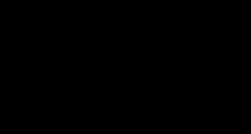
\includegraphics[width=\columnwidth]{FIGURA.png}
	\caption{Resistance R$_{x}$ as a function of I$_{DN3}$}
	\label{fig.example}
\end{figure}
\begin{table}[h]\tiny
	\centering
	\caption{Table caption.}
	\label{table.Ex}
	\begin{tabular}{c c c}	
		\hline	
		Device& Measured (x10\textsuperscript{-5}A/cm\textsuperscript{2})& Modeled (x10\textsuperscript{-5}A/cm\textsuperscript{2})\\
		\hline
		1&12.47&12.74\\
		2&12.46&12.64\\
		3&12.45&12.54\\
		4&12.44&12.44\\
		\hline
	\end{tabular}
\end{table}

\section{Let's try more pages}
\lipsum

\lipsum

\lipsum

\lipsum

\lipsum

\lipsum

\lipsum

\lipsum

\lipsum

\lipsum

\lipsum

\lipsum

\lipsum

\lipsum
% ACKNOWLEDGEMENTS SECTION
\setcounter{secnumdepth}{0}
\section{Acknowledgements}
The authors would like to acknowledge...
% BILIOGRAPHY SECTION
\bibliographystyle{IEEEtran}
\bibliography{IEEEabrv,BibJICS}% Second term corresponds to the file where your bibliography is saved.
\end{document}
%% That's all, folks